\subsection{One-way forwarding}

%----------------------------------
\subsubsection{1 Gbps Test Results}

\begin{table}[h!]
\centering
\caption{Results of one-way 1 Gbit/s of 64-byte frames}
\begin{tabular}{|l|r|r|r|r|r|r|}
\hline
\multicolumn{1}{|c|}{\textbf{Config}} &
\multicolumn{1}{c|}{\textbf{Energy [Wh] }} &
\multicolumn{1}{c|}{\textbf{Pkt Loss [\%]}} &
\multicolumn{1}{c|}{\textbf{Avg Lat [$\mu$s]}} &
\multicolumn{1}{c|}{\textbf{Jitter [$\mu$s]}} \\
\hline 
VPP-1 & 5.68 & 0.00 & 12.8 & 9.5 \\
VPP-4 & 6.46 & 0.00 & 27.45 & 13.55 \\
VPP-10 & 7.86 & 0.00 & 28.3 & 12.65 \\
Linux & 6.78 & 0.00 & 108.05 & 97.25 \\
\hline
\end{tabular}
\label{tab:1udp:64B}
\end{table}


%------------------------------------------------------
\begin{table}[h!]
\centering
\caption{Results of one-way 1 Gbit/s of 512-byte frames}
\begin{tabular}{|l|r|r|r|r|r|r|}
\hline
\multicolumn{1}{|c|}{\textbf{Config}} &
\multicolumn{1}{c|}{\textbf{Energy [Wh] }} &
\multicolumn{1}{c|}{\textbf{Pkt Loss [\%]}} &
\multicolumn{1}{c|}{\textbf{Avg Lat [$\mu$s]}} &
\multicolumn{1}{c|}{\textbf{Jitter [$\mu$s]}} \\
\hline 
VPP-1 & 5,69 & 0.00 & 12.1 & 11.7 \\
VPP-4 & 6.48 & 0.00 & 22.85 & 17.4 \\
VPP-10 & TODO &  &  &  \\
Linux & 6.23 & 0.00 & 56.1 & 51.35 \\
\hline
\end{tabular}
\label{tab:1udp:512B}
\end{table}


%------------------------------------------------------
\begin{table}[h!]
\centering
\caption{Results of one-way 1 Gbit/s of 889-byte frames}
\begin{tabular}{|l|r|r|r|r|r|r|}
\hline
\multicolumn{1}{|c|}{\textbf{Config}} &
\multicolumn{1}{c|}{\textbf{Energy [Wh] }} &
\multicolumn{1}{c|}{\textbf{Pkt Loss [\%]}} &
\multicolumn{1}{c|}{\textbf{Avg Lat [$\mu$s]}} &
\multicolumn{1}{c|}{\textbf{Jitter [$\mu$s]}} \\
\hline 
VPP-1 & 5,76 & 0.00 & 10.3 & 8.4 \\
VPP-4 & 6.45 & 0.00 & 21.3 & 17.6 \\
VPP-10 & 7.85 & 0.00 & 20.95 & 16.3  \\
Linux & TODO &  &  &  \\
\hline
\end{tabular}
\label{tab:1udp:889B}
\end{table}


%------------------------------------------------------
\begin{table}[h!]
\centering
\caption{Results of one-way 1 Gbit/s of 1280-byte frames}
\begin{tabular}{|l|r|r|r|r|r|r|}
\hline
\multicolumn{1}{|c|}{\textbf{Config}} &
\multicolumn{1}{c|}{\textbf{Energy [Wh] }} &
\multicolumn{1}{c|}{\textbf{Pkt Loss [\%]}} &
\multicolumn{1}{c|}{\textbf{Avg Lat [$\mu$s]}} &
\multicolumn{1}{c|}{\textbf{Jitter [$\mu$s]}} \\
\hline 
VPP-1 & TODO &  &  &  \\
VPP-4 & 6.46 & 0.00 & 18.3 & 17.2 \\
VPP-10 & 7.84 & 0.00 & 18.8 & 15.95  \\
Linux & TODO &  &  &  \\
\hline
\end{tabular}
\label{tab:1udp:1280B}
\end{table}


%------------------------------------------------------
\begin{table}[h!]
\centering
\caption{Results of one-way 1 Gbit/s of 1518-byte frames}
\begin{tabular}{|l|r|r|r|r|r|r|}
\hline
\multicolumn{1}{|c|}{\textbf{Config}} &
\multicolumn{1}{c|}{\textbf{Energy [Wh] }} &
\multicolumn{1}{c|}{\textbf{Pkt Loss [\%]}} &
\multicolumn{1}{c|}{\textbf{Avg Lat [$\mu$s]}} &
\multicolumn{1}{c|}{\textbf{Jitter [$\mu$s]}} \\
\hline 
VPP-1 & 5.66 & 0.00 & 7.2 & 5.5  \\
VPP-4 & 6.42 & 0.00 & 16.1 & 15.75 \\
VPP-10 & 7.84 & 0.00 & 18.8 & 15.95 \\
Linux & TODO &  &  &  \\
\hline
\end{tabular}
\label{tab:1udp:1518B}
\end{table}

%---------------------------------------------------------------------------------------------
%---------------------------------------------------------------------------------------------
%---------------------------------------------------------------------------------------------
\subsubsection{10 Gbps Test Results}

As shown in Tab.~\ref{tab:10udp:64B}, both VPP-1 and the Linux stack were unable to handle this packet rate at 10~Gbit/s with 64-byte frames, resulting in high packet loss and significantly increased latency. 
VPP-4 managed to process the traffic with minimal loss, achieving the lowest latency and jitter among all configurations. 
VPP-10 also completed the test losslessly, but with slightly higher latency. 

%------------------------------------------------------
\begin{table}[h!]
\centering
\caption{Results of one-way 10 Gbit/s of 64-byte frames}
\begin{tabular}{|l|r|r|r|r|r|r|}
\hline
\multicolumn{1}{|c|}{\textbf{Config}} &
\multicolumn{1}{c|}{\textbf{Energy [Wh] }} &
\multicolumn{1}{c|}{\textbf{Pkt Loss [\%]}} &
\multicolumn{1}{c|}{\textbf{Avg Lat [$\mu$s]}} &
\multicolumn{1}{c|}{\textbf{Jitter [$\mu$s]}} \\
\hline 
VPP-1 & 5.72 & 59.5 & 589.50 & 14.05 \\
VPP-4 & 6.56 & 0.02 & 20.60 & 6.00 \\
VPP-10 & 8.04 & 0.00 & 30.00 & 12.90 \\
Linux & 7.35 & 80.97 & 3846.30 & 217.8 \\
\hline
\end{tabular}
\label{tab:10udp:64B}
\end{table}

It can be seen from Tab.~\ref{tab:10udp:512B} that increasing the frame size to 512~bytes allowed all tested configurations to handle the traffic without packet loss. 
Although the latency of the Linux stack improved significantly compared to the previous measurement, it still remained the highest among all configurations.
The energy consumption of the Linux configuration decreased, likely due to reduced overhead from system calls.

%------------------------------------------------------
\begin{table}[h!]
\centering
\caption{Results of one-way 10 Gbit/s of 512-byte frames}
\begin{tabular}{|l|r|r|r|r|r|r|}
\hline
\multicolumn{1}{|c|}{\textbf{Config}} &
\multicolumn{1}{c|}{\textbf{Energy [Wh] }} &
\multicolumn{1}{c|}{\textbf{Pkt Loss [\%]}} &
\multicolumn{1}{c|}{\textbf{Avg Lat [$\mu$s]}} &
\multicolumn{1}{c|}{\textbf{Jitter [$\mu$s]}} \\
\hline 
VPP-1 & 5.60 & 0.00 & 19.95 & 12.00 \\
VPP-4 & 6.48 & 0.00 & 28.20 & 14.50 \\
VPP-10 & 7.97 & 0.00 & 29.05 & 13.65 \\
Linux & 6.85 & 0.00 & 129.4 & 99.35 \\
\hline
\end{tabular}
\label{tab:10udp:512B}
\end{table}

In this test with 889-byte frames, all VPP configurations show similar results to the previous measurement, although with slightly increased jitter.
This may be due to VPP constructing processing vectors based on the number of packets rather than their total size.
The increased frame size improved Linux's average latency, possibly due to reduced per-packet processing overhead.
The discussed results are summarized in Table~\ref{tab:10udp:889B}.

%------------------------------------------------------
\begin{table}[h!]
\centering
\caption{Results of one-way 10 Gbit/s of 889-byte frames}
\begin{tabular}{|l|r|r|r|r|r|r|}
\hline
\multicolumn{1}{|c|}{\textbf{Config}} &
\multicolumn{1}{c|}{\textbf{Energy [Wh] }} &
\multicolumn{1}{c|}{\textbf{Pkt Loss [\%]}} &
\multicolumn{1}{c|}{\textbf{Avg Lat [$\mu$s]}} &
\multicolumn{1}{c|}{\textbf{Jitter [$\mu$s]}} \\
\hline 
VPP-1 & 5.62 & 0.00 & 23.4 & 14.95 \\
VPP-4 & 6.48 & 0.00 & 26.5 & 18.25 \\
VPP-10 & 7.95 & 0.00 & 26.95 & 17.55 \\
Linux & 6.67 & 0.00 & 66.45 & 68.3 \\
\hline
\end{tabular}
\label{tab:10udp:889B}
\end{table}

As shown in Table~\ref{tab:10udp:1280B}, the VPP configurations performed similarly to the previous measurement.
In contrast, Linux achieved slightly improved latency and jitter, potentially due to the larger frame size further reducing per-packet processing overhead. 

%------------------------------------------------------
\begin{table}[h!]
\centering
\caption{Results of one-way 10 Gbit/s of 1280-byte frames}
\begin{tabular}{|l|r|r|r|r|r|r|}
\hline
\multicolumn{1}{|c|}{\textbf{Config}} &
\multicolumn{1}{c|}{\textbf{Energy [Wh] }} &
\multicolumn{1}{c|}{\textbf{Pkt Loss [\%]}} &
\multicolumn{1}{c|}{\textbf{Avg Lat [$\mu$s]}} &
\multicolumn{1}{c|}{\textbf{Jitter [$\mu$s]}} \\
\hline 
VPP-1 & 5.58 & 0.00 & 22.8 & 17.05 \\
VPP-4 & 6.47 & 0.00 & 25.95 & 16.90 \\
VPP-10 & 7.98 & 0.00 & 26.80 & 16.60 \\
Linux & 6.54 & 0.00 & 57.05 & 65.50 \\
\hline
\end{tabular}
\label{tab:10udp:1280B}
\end{table}

The results for 1518-byte frames are consistent with those observed at 1280 bytes, with no significant improvements in consumption, latency, or jitter.
This suggests that increasing the frame size beyond 1280 bytes does not bring further performance gains in the tested configurations.
The detailed results are presented in Table~\ref{tab:10udp:1518B}.

%------------------------------------------------------
\begin{table}[h!]
\centering
\caption{Results of one-way 10 Gbit/s of 1518-byte frames}
\begin{tabular}{|l|r|r|r|r|r|r|}
\hline
\multicolumn{1}{|c|}{\textbf{Config}} &
\multicolumn{1}{c|}{\textbf{Energy [Wh] }} &
\multicolumn{1}{c|}{\textbf{Pkt Loss [\%]}} &
\multicolumn{1}{c|}{\textbf{Avg Lat [$\mu$s]}} &
\multicolumn{1}{c|}{\textbf{Jitter [$\mu$s]}} \\
\hline 
VPP-1 & 5.57 & 0.00 & 20.45 & 14.95 \\
VPP-4 & 6.48 & 0.00 & 24.00 & 17.45 \\
VPP-10 & 7.97 & 0.00 & 25.40 & 17.70 \\
Linux & 6.51 & 0.00 & 61.75 & 65.80 \\
\hline
\end{tabular}
\label{tab:10udp:1518B}
\end{table}

Figure~\ref{fig:10g} shows the energy efficiency of each configuration in this test in terms of delivered packets and bytes.
The significant drop in performance for VPP-1 and Linux in 64-byte frames test is caused by large packet loss.
When all packets are successfully delivered, all VPP configurations maintain stable BPWh values, which is due to their busy-wait processing model.
The Linux stack, on the other hand, becomes more efficient with increasing frame size, likely as a result of less frequent system calls.

\begin{figure}[!htbp]
    \centering
    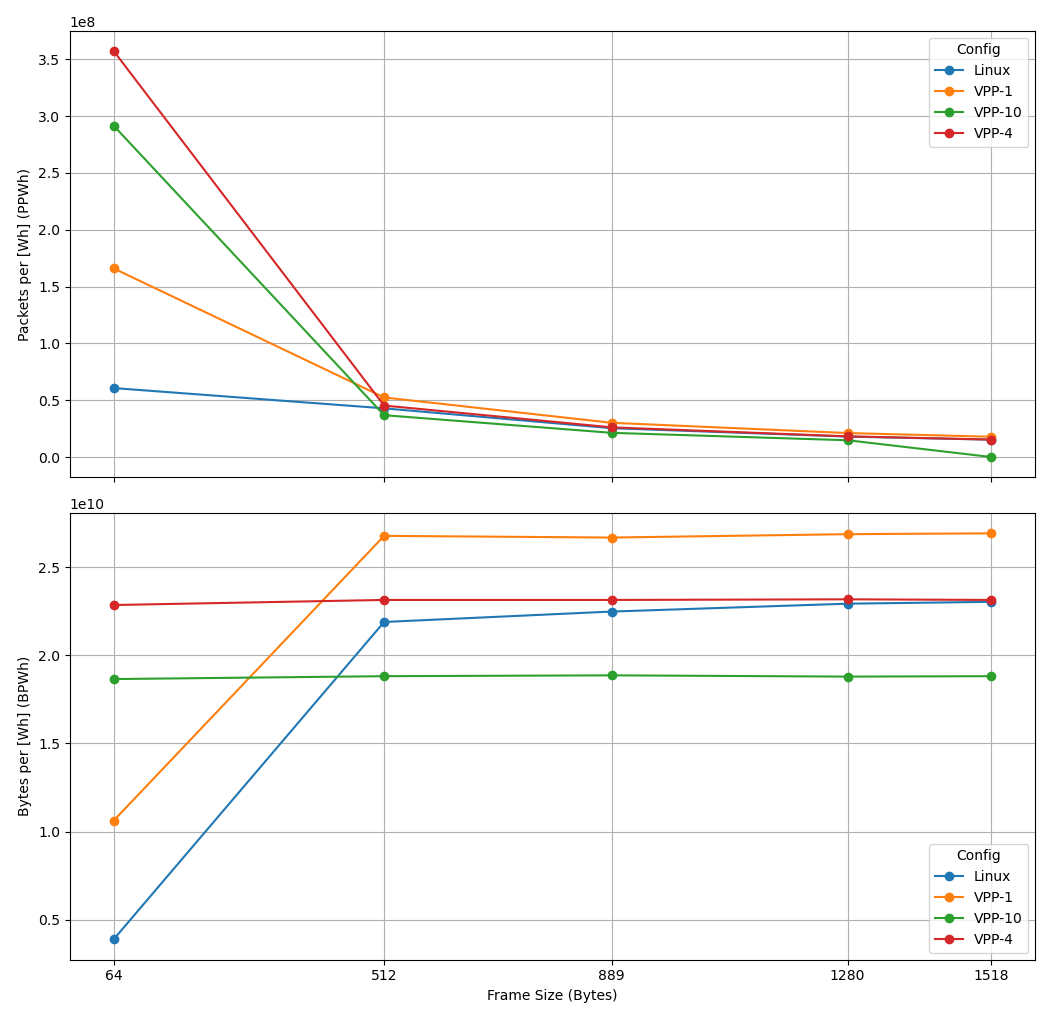
\includegraphics[width=\linewidth]{images/consumption-10g.png}
    \caption{Energy efficiency per delivered data in one-way 10\,Gbit/s.}
    \label{fig:10g}
\end{figure}



%---------------------------------------------------------------------------------------------
%---------------------------------------------------------------------------------------------
%---------------------------------------------------------------------------------------------
\subsubsection{25 Gbps Test Results}

As shown in Table~\ref{tab:25udp:64B}, none of the configurations were able to deliver all data.
In all VPP setups, the delivered data maintained low jitter,
likely due to lost packets in RX queues being overwritten by fresher incoming traffic.
This stress test also demonstrates that the Linux stack is unable to handle such network load, resulting in extremely high latency of delivered packets.
These results highlight the advantages of VPP under heavy traffic conditions.

%------------------------------------------------------
\begin{table}[h!]
\centering
\caption{Results of one-way 25 Gbit/s of 64-byte frames}
\begin{tabular}{|l|r|r|r|r|r|r|}
\hline
\multicolumn{1}{|c|}{\textbf{Config}} &
\multicolumn{1}{c|}{\textbf{Energy [Wh] }} &
\multicolumn{1}{c|}{\textbf{Pkt Loss [\%]}} &
\multicolumn{1}{c|}{\textbf{Avg Lat [$\mu$s]}} &
\multicolumn{1}{c|}{\textbf{Jitter [$\mu$s]}} \\
\hline 
VPP-1 & 5.59 & 83.29 & 577.5 & 7.70 \\
VPP-4 & 6.56 & 49.00 & 198.85 & 7.65 \\
VPP-10 & 8.26 & 29.55 & 155.35 & 11.95 \\
Linux & 7.43 & 92.71 & 5597.95 & 632.00 \\
\hline
\end{tabular}
\label{tab:25udp:64B}
\end{table}

When the frame size increased to 512 bytes, all VPP configurations were able to deliver the full traffic,
except for VPP-1, which dropped a negligible amount of packets.
All VPP setups showed reduced latency and jitter compared to the previous test.
The Linux stack, however, was still unable to handle the traffic, dropping nearly 50\% of the packets and showing extremely high latency in the delivered traffic,
as summarized in Table~\ref{tab:25udp:512B}.

%------------------------------------------------------
\begin{table}[h!]
\centering
\caption{Results of one-way 25 Gbit/s of 512-byte frames}
\begin{tabular}{|l|r|r|r|r|r|r|}
\hline
\multicolumn{1}{|c|}{\textbf{Config}} &
\multicolumn{1}{c|}{\textbf{Energy [Wh] }} &
\multicolumn{1}{c|}{\textbf{Pkt Loss [\%]}} &
\multicolumn{1}{c|}{\textbf{Avg Lat [$\mu$s]}} &
\multicolumn{1}{c|}{\textbf{Jitter [$\mu$s]}} \\
\hline 
VPP-1 & 5.57 & 0.07 & 31.85 & 11.15 \\
VPP-4 & 6.43 & 0.00 & 29.55 & 13.75 \\
VPP-10 & 8.03 & 0.00 & 31.00 & 14.45 \\
Linux & 7.57 & 47.97 & 7819.60 & 477.55 \\
\hline
\end{tabular}
\label{tab:25udp:512B}
\end{table}

As indicated by the results in Table~\ref{tab:25udp:889B}, the VPP-1 configuration achieved lower latency, likely due to the absence of packet drops.
Even when an average packet size was used, the Linux stack was still unable to deliver all packets, with measurable losses.
This likely contributed to the relatively high latency and jitter observed in the Linux configuration.

%------------------------------------------------------
\begin{table}[h!]
\centering
\caption{Results of one-way 25 Gbit/s of 889-byte frames}
\begin{tabular}{|l|r|r|r|r|r|r|}
\hline
\multicolumn{1}{|c|}{\textbf{Config}} &
\multicolumn{1}{c|}{\textbf{Energy [Wh] }} &
\multicolumn{1}{c|}{\textbf{Pkt Loss [\%]}} &
\multicolumn{1}{c|}{\textbf{Avg Lat [$\mu$s]}} &
\multicolumn{1}{c|}{\textbf{Jitter [$\mu$s]}} \\
\hline 
VPP-1 & 5.67 & 0.00 & 23.45 & 11.15 \\
VPP-4 & 6.39 & 0.00 & 30.50 & 15.50 \\
VPP-10 & 8.01 & 0.00 & 29.45 & 15.55 \\
Linux & 7.42 & 0.87 & 166.05 & 111.15 \\
\hline
\end{tabular}
\label{tab:25udp:889B}
\end{table}

In this test, using 1280-byte frames, all configurations were able to deliver the complete dataset.
Without exception, all VPP configurations achieved results comparable to the previous measurement.
The use of larger frames had a positive impact on latency in the Linux configuration,
as indicated by the results in Table~\ref{tab:25udp:1280B}.

%------------------------------------------------------
\begin{table}[h!]
\centering
\caption{Results of one-way 25 Gbit/s of 1280-byte frames}
\begin{tabular}{|l|r|r|r|r|r|r|}
\hline
\multicolumn{1}{|c|}{\textbf{Config}} &
\multicolumn{1}{c|}{\textbf{Energy [Wh] }} &
\multicolumn{1}{c|}{\textbf{Pkt Loss [\%]}} &
\multicolumn{1}{c|}{\textbf{Avg Lat [$\mu$s]}} &
\multicolumn{1}{c|}{\textbf{Jitter [$\mu$s]}} \\
\hline 
VPP-1 & 5.68 & 0.00 & 23.85 & 10.30 \\
VPP-4 & 6.48 & 0.00 & 31.15 & 15.40 \\
VPP-10 & 7.98 & 0.00 & 28.40 & 16.15 \\
Linux & 7.10  & 0.00 & 146.90 & 126.20 \\
\hline
\end{tabular}
\label{tab:25udp:1280B}
\end{table}

As indicated by the results in Table~\ref{tab:25udp:1518B}, increasing the frame size to the maximum had no impact on performance compared to the previous measurement.
Only the Linux stack showed slightly better results in terms of latency and jitter.

%------------------------------------------------------
\begin{table}[h!]
\centering
\caption{Results of one-way 25 Gbit/s of 1518-byte frames}
\begin{tabular}{|l|r|r|r|r|r|r|}
\hline
\multicolumn{1}{|c|}{\textbf{Config}} &
\multicolumn{1}{c|}{\textbf{Energy [Wh] }} &
\multicolumn{1}{c|}{\textbf{Pkt Loss [\%]}} &
\multicolumn{1}{c|}{\textbf{Avg Lat [$\mu$s]}} &
\multicolumn{1}{c|}{\textbf{Jitter [$\mu$s]}} \\
\hline 
VPP-1 & 5.70 & 0.00 & 24.45 & 14.90 \\
VPP-4 & 6.46 & 0.00 & 30.60 & 15.80 \\
VPP-10 & 7.96 & 0.00 & 28.9 & 15.65 \\
Linux & 7.00  & 0.00 & 130.00 & 105.30 \\
\hline
\end{tabular}
\label{tab:25udp:1518B}
\end{table}


Figure~\ref{fig:25g} illustrates the energy efficiency of each configuration in terms of delivered packets and bytes.
Compared to the previous test, the Linux stack performed significantly worse, while VPP maintained stable BPWh, except in the case of 64-byte frames.

\begin{figure}[!htbp]
    \centering
    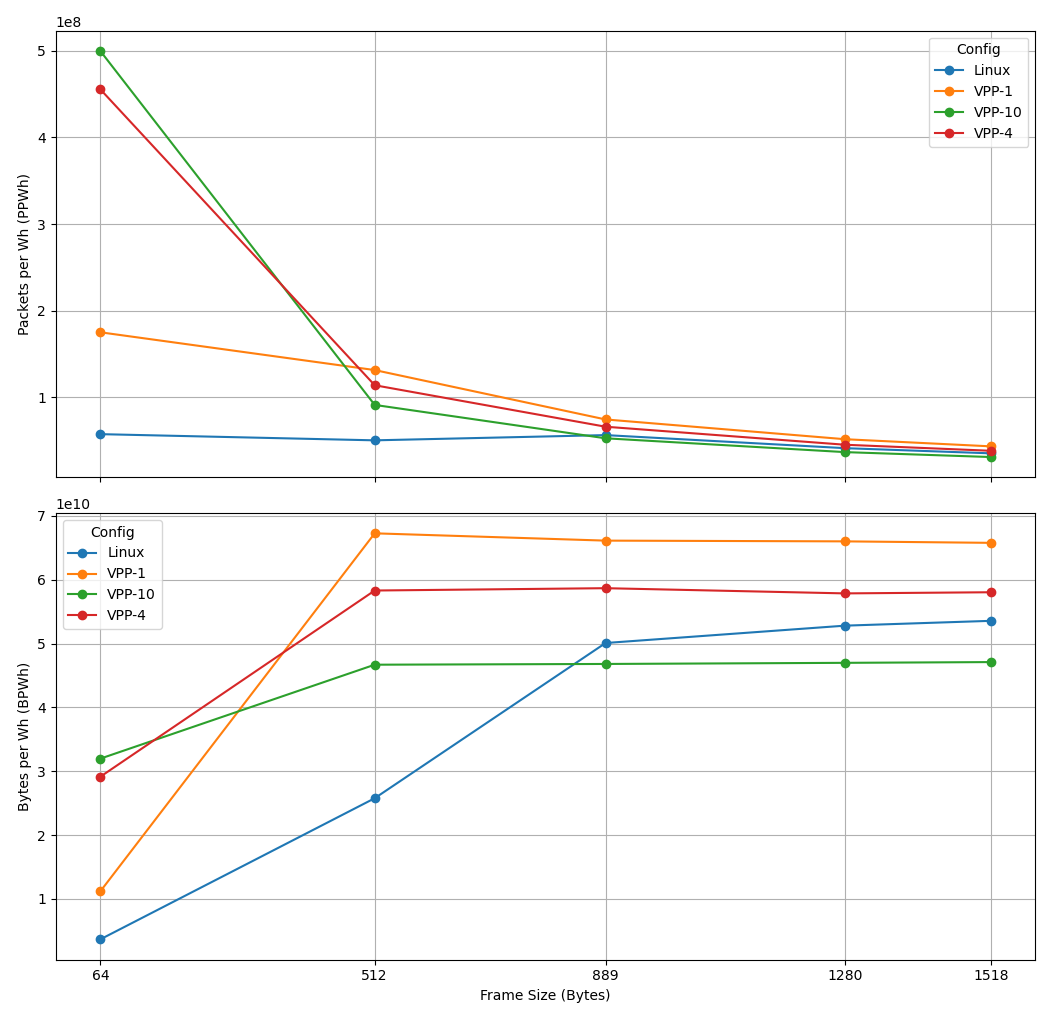
\includegraphics[width=\linewidth]{images/consumption-25g.png}
    \caption{Energy efficiency per delivered data in one-way 25\,Gbit/s.}
    \label{fig:25g}
\end{figure}


%-----------------------------------
\subsubsection{40 Gbps Test Results}

The results of the 40Gbit/s test, summarized in Table\ref{tab:40udp:64B}, clearly show that all configurations struggled to process the traffic.
The performance was comparable to the 25~Gbit/s test with 64-byte frames, but with even higher packet loss rates -- with the Linux stack delivering less than 5\% of the packets.

%------------------------------------------------------
\begin{table}[h!]
\centering
\caption{Results of one-way 40 Gbit/s of 64-byte frames}
\begin{tabular}{|l|r|r|r|r|r|r|}
\hline
\multicolumn{1}{|c|}{\textbf{Config}} &
\multicolumn{1}{c|}{\textbf{Energy [Wh] }} &
\multicolumn{1}{c|}{\textbf{Pkt Loss [\%]}} &
\multicolumn{1}{c|}{\textbf{Avg Lat [$\mu$s]}} &
\multicolumn{1}{c|}{\textbf{Jitter [$\mu$s]}} \\
\hline 
VPP-1 & 5.60 & 89.53 & 576.00 & 6.50 \\
VPP-4 & 6.57 & 67.54 & 195.70 & 6.57 \\
VPP-10 & 8.12 & 54.38 & 152.05 & 9.20 \\
Linux & 7.34 & 95.43 & 5629.05 & 550.30 \\
\hline
\end{tabular}
\label{tab:40udp:64B}
\end{table}

As the results in Table~\ref{tab:40udp:512B} suggest, only the VPP-1 and Linux configurations were unable to deliver all data,
while VPP-4 and VPP-10 showed significant improvements in latency.
The average latency of the Linux stack increased, which may be attributed to a larger number of packets being successfully delivered.

%------------------------------------------------------
\begin{table}[h!]
\centering
\caption{Results of one-way 40 Gbit/s of 512-byte frames}
\begin{tabular}{|l|r|r|r|r|r|r|}
\hline
\multicolumn{1}{|c|}{\textbf{Config}} &
\multicolumn{1}{c|}{\textbf{Energy [Wh] }} &
\multicolumn{1}{c|}{\textbf{Pkt Loss [\%]}} &
\multicolumn{1}{c|}{\textbf{Avg Lat [$\mu$s]}} &
\multicolumn{1}{c|}{\textbf{Jitter [$\mu$s]}} \\
\hline 
VPP-1 & 5.82 & 35.26 & 292.45 & 122.15 \\
VPP-4 & 6.56 & 0.00 & 28.80 & 9.90 \\
VPP-10 & 8.00 & 0.00 & 35.45 & 14.35 \\
Linux & TODO &  &  &  \\
\hline
\end{tabular}
\label{tab:40udp:512B}
\end{table}

In the 889-byte frame test, the results for VPP-4 and VPP-10 remained consistent with the previous experiment.
VPP-1 was almost able to handle the full traffic, while the Linux stack managed to process only about half of the data -- and did so with extremely high latency.
The results are summarized in Table~\ref{tab:40udp:889B}.

%------------------------------------------------------
\begin{table}[h!]
\centering
\caption{Results of one-way 40 Gbit/s of 889-byte frames}
\begin{tabular}{|l|r|r|r|r|r|r|}
\hline
\multicolumn{1}{|c|}{\textbf{Config}} &
\multicolumn{1}{c|}{\textbf{Energy [Wh] }} &
\multicolumn{1}{c|}{\textbf{Pkt Loss [\%]}} &
\multicolumn{1}{c|}{\textbf{Avg Lat [$\mu$s]}} &
\multicolumn{1}{c|}{\textbf{Jitter [$\mu$s]}} \\
\hline 
VPP-1 & 5.77 & 3.85 & 203.05 & 25.2 \\
VPP-4 & 6.54 & 0.00 & 32.55 & 13.75 \\
VPP-10 & 8.00 & 0.00 & 33.60 & 18.50 \\
Linux & 7.63 & 49.85 & 7222.80 & 315.40 \\
\hline
\end{tabular}
\label{tab:40udp:889B}
\end{table}

As the data in Table~\ref{tab:40udp:1280B} suggest, all VPP configurations performed similarly to the corresponding 25~Gbit/s test,
with the exception of VPP-1, which showed higher latency likely due to the increased traffic load.
The Linux stack was almost able to process all data, showing a significant improvement compared to the 889-byte frame test.

%------------------------------------------------------
\begin{table}[h!]
\centering
\caption{Results of one-way 40 Gbit/s of 1280-byte frames}
\begin{tabular}{|l|r|r|r|r|r|r|}
\hline
\multicolumn{1}{|c|}{\textbf{Config}} &
\multicolumn{1}{c|}{\textbf{Energy [Wh] }} &
\multicolumn{1}{c|}{\textbf{Pkt Loss [\%]}} &
\multicolumn{1}{c|}{\textbf{Avg Lat [$\mu$s]}} &
\multicolumn{1}{c|}{\textbf{Jitter [$\mu$s]}} \\
\hline 
VPP-1 & 5.79 & 0.00 & 32.50 & 14.65 \\
VPP-4 & 6.40 & 0.00 & 33.95 & 14.35 \\
VPP-10 & 8.02 & 0.00 & 32.15 & 16.85 \\
Linux & 7.59 & 6.25 & 2830.95 & 104.1 \\
\hline
\end{tabular}
\label{tab:40udp:1280B}
\end{table}

The data in Table~\ref{tab:40udp:1518B} demonstrate that the VPP configurations returned results comparable to the 1280-byte frame test,
indicating that the architecture has already reached its efficiency limit under the tested conditions.
In contrast, the Linux stack benefited from the increased frame size, being able to almost deliver the full traffic volume with significantly reduced latency.

%------------------------------------------------------
\begin{table}[h!]
\centering
\caption{Results of one-way 40 Gbit/s of 1518-byte frames}
\begin{tabular}{|l|r|r|r|r|r|r|}
\hline
\multicolumn{1}{|c|}{\textbf{Config}} &
\multicolumn{1}{c|}{\textbf{Energy [Wh] }} &
\multicolumn{1}{c|}{\textbf{Pkt Loss [\%]}} &
\multicolumn{1}{c|}{\textbf{Avg Lat [$\mu$s]}} &
\multicolumn{1}{c|}{\textbf{Jitter [$\mu$s]}} \\
\hline 
VPP-1 & 5.83 & 0.00 & 30.35 & 15.75 \\
VPP-4 & 6.43 & 0.00 & 34.20 & 14.75 \\
VPP-10 & 8.02 & 0.00 & 33.30 & 14.80 \\
Linux & 7.36 & 0.08 & 195.05 & 122.05 \\
\hline
\end{tabular}
\label{tab:40udp:1518B}
\end{table}






%-------------------------------------------------------------------------------
\subsection{Bidirectional UDP 1 Gbit/s}
TOTO ODSTRANIT!!!!\\
zatím ponecháno jen kvůli úvodu\\

This section presents a set of performance and efficiency tests performed on the Device Under Test (DUT) using bidirectional UDP traffic at a total rate of 1\,Gbit/s. 
The goal is to evaluate the forwarding performance of the DUT under varying packet sizes, simulating realistic traffic patterns with increasing stress on the packet-processing path.

To provide a comprehensive and representative view, the tests are structured into five subsections, each corresponding to a different Ethernet frame size. 
Four of the selected sizes -- 64 bytes, 512 bytes, 1280 bytes, and 1518 bytes -- are recommended by RFC2544\cite{rfc2544} 
covering both edge-cases and practically relevant intermediate values. 
The fifth size, 889 bytes, was chosen because it was identified as the average size in real-world network traffic by Jurkiewicz et al.~\cite{JURKIEWICZ202115}. 
This selection covers the full range of standard Ethernet frame sizes, from the minimum to the maximum non-jumbo frames, 
and includes a representative average frame size observed in real network traffic.

Traffic in all scenarios is generated using TRex with the \textit{udp\_1pkt\_src\_ip\_split.py} profile, 
which ensures that each packet carries a unique source IP address to simulate multiple concurrent clients, while maintaining a single destination IP per direction. 
The routing table of the DUT contains only two active forwarding entries, corresponding to the test routes, in addition to two administrative entries used for management.
The total offered load is 1\,Gbit/s, symmetrically split between both directions (500\,Mbit/s each).
The chosen load of 1 Gbit/s is representative of a realistic aggregate traffic pattern that could be observed in a small or medium-sized enterprise network, especially when routed through a central gateway.

The DUT is configured with the Vector Packet Processing (VPP) stack and tested under three levels of parallelism: using 1, 4, and 10 worker threads. 
The number of RX/TX queues is aligned with the number of active worker threads in each configuration to ensure balanced packet distribution and optimal resource utilization.

To provide a baseline for comparison, all scenarios are also executed using the standard Linux kernel networking stack, 
configured with equivalent routing and interface parameters, but able to use all 20 cores of CPU. 
This allows for a direct comparison between VPP and traditional kernel-based forwarding in terms of performance and energy efficiency.

The aim of this test is to observe the behavior of the VPP forwarding plane under low traffic load of small packets and to evaluate its energy efficiency.

%-------------------------------------------------------------------------------
\subsubsection{64-bytes frames}
This test evaluates the behavior of the VPP forwarding plane under a low-throughput traffic load composed of minimum-sized Ethernet frames (64 bytes). 
Such frames result in a high packet-per-second rate for a given bandwidth, which increases the processing overhead per bit of data. 
This configuration represents a stress scenario for packet forwarding and allows assessment of the system’s efficiency in handling a large number of small packets.

\begin{table}[h!]
\centering
\begin{tabular}{|l|r|r|r|}
\hline
\multicolumn{1}{|c|}{\textbf{Configuration}} &
\multicolumn{1}{c|}{\textbf{Watts used}} &
\multicolumn{1}{c|}{\textbf{PPW}} &
\multicolumn{1}{c|}{\textbf{BPW}} \\
\hline
VPP -- 1 worker & 848.08 & 20 726 965.60 & 1 326 525 798.50 \\
VPP -- 4 workers & 951.03 & 18 483 249.76 & 1 182 927 982.40 \\
VPP -- 10 workers & 1 193.56 & 14 727 474.94 & 942 558 396.09 \\
Linux stack & 1 257.25 & 13 981 407.81 & 894 810 100.29 \\
\hline
\end{tabular}
\caption{Result of Bidirectional UDP 1 Gbit/s of 64-bytes packets test}
\label{tab:udp:one}
\end{table}

As the results in Table \ref{tab:udp:one} show, the power consumption increases notably with the number of worker threads in the VPP stack. 
While all VPP configurations deliver identical packet and byte throughput, the most energy-efficient setup in this measurement is the single-worker variant, consuming roughly 850 Watts during the test. 
In contrast, the traditional Linux network stack demonstrates the highest energy usage, despite handling the same volume of packets.

This discrepancy can likely be attributed to the cost of processing a high number of small packets in kernel space. 
Since the test uses fixed-size 64-byte frames, which are known to generate frequent system calls and context switches in Linux, 
the forwarding path becomes less efficient compared to VPP’s user-space architecture, where such overheads are significantly reduced. 
The results highlight the energy cost of kernel-based packet forwarding in scenarios dominated by small-packet traffic.

%------------------------------------------------------------------------------
\subsubsection{512-bytes frames}
This test focuses on the forwarding performance of the VPP data plane when processing medium-sized Ethernet frames of 512 bytes. 
These frames offer a balance between protocol overhead and payload efficiency and are representative of many real-world applications that do not utilize maximum frame sizes. 
The test helps to evaluate how the system handles typical traffic patterns with moderate packet rates and processing demands.

Notably, the 554-byte frame size (512 bytes of data) represents the historical maximum size of a DNS response over UDP without the use of extension mechanisms such as EDNS(0).\cite{satrapa2023dns} 

\begin{table}[h!]
\centering
\begin{tabular}{|l|r|r|r|}
\hline
\multicolumn{1}{|c|}{\textbf{Configuration}} &
\multicolumn{1}{c|}{\textbf{Watts used}} &
\multicolumn{1}{c|}{\textbf{PPW}} &
\multicolumn{1}{c|}{\textbf{BPW}} \\
\hline
VPP -- 1 worker & 851.21 & 2 581 343.78 & 1 321 648 015.98 \\
VPP -- 4 workers & 969.49 & 2 266 413.93 & 1 160 403 931.63 \\
VPP -- 10 workers & 1 175.07 & 1 869 901.91 & 957 389 779.06 \\
Linux stack & 965.58 & 2 275 591.60 & 1 165 102 847.70 \\
\hline
\end{tabular}
\caption{Result of Bidirectional UDP 1 Gbit/s of 512-bytes frames test}
\label{tab:udp:two}
\end{table}

As seen in the result Table \ref{tab:udp:two}, the power consumption of VPP remains stable. 
On the other hand, compared to the 64-byte scenario, the Linux stack shows improved energy efficiency when handling 512-byte packets. 
This is primarily due to the lower packet-per-second (PPS) rate associated with larger frames, which reduces the overhead caused by frequent context switches and system calls in the kernel space. 
Although the Linux stack remains slightly less efficient than VPP with one worker in this scenario, the margin is smaller than in the minimum-packet-size test.

%------------------------------------------------------------------------------
\subsubsection{889-bytes frames}
This test focuses on the forwarding performance of the VPP data plane when processing medium-sized Ethernet frames of 889 bytes. 
These frames offer a favorable balance between protocol overhead and payload efficiency. 
As mentioned earlier, this size was identified as the average frame size observed in real-world network traffic, according to a study by Jurkiewicz et al.~\cite{JURKIEWICZ202115}.

The test helps evaluate how the system handles traffic patterns that more closely resemble typical production environments, where packet sizes vary but tend to concentrate around this average. 
Compared to minimum-sized or maximum-sized frames, the 889-byte frame represents a realistic mid-point for both packet rate and processing complexity.

\begin{table}[h!]
\centering
\begin{tabular}{|l|r|r|r|}
\hline
\multicolumn{1}{|c|}{\textbf{Configuration}} &
\multicolumn{1}{c|}{\textbf{Watts used}} &
\multicolumn{1}{c|}{\textbf{PPW}} &
\multicolumn{1}{c|}{\textbf{BPW}} \\
\hline
VPP -- 1 worker & 853.27 & 1 483 079.03 & 1 318 457 253.58 \\
VPP -- 4 workers & 952.46 & 1 328 629.91 & 1 181 151 986.18 \\
VPP -- 10 workers & 1 190.42 & 1 063 042.32 & 945 044 623.54 \\
Linux stack & 940.33 & 1 345 768.87 & 1 196 388 523.99 \\
\hline
\end{tabular}
\caption{Result of Bidirectional UDP 1 Gbit/s of 889-bytes frames test}
\label{tab:udp:three}
\end{table}

As shown in Table \ref{tab:udp:three}, the third test with 889-byte frames, 
VPP's power consumption remains stable across different worker thread configurations. 
In the case of the Linux stack, energy efficiency improves slightly compared to the previous (512-byte) test, though the difference is minimal. 
The change is significantly smaller than the improvement observed between the 64-byte and 512-byte scenarios, suggesting that the impact of increasing frame size becomes less pronounced beyond a certain point.

%-------------------------------------------------------------------------------
\subsubsection{1280-bytes frames}
This test focuses on the forwarding performance of the VPP data plane when processing large Ethernet frames of 1280 bytes. 
These frames represent a size commonly used in environments where larger payloads are transferred, but without exceeding the typical Ethernet MTU limit of 1500 bytes. 
This size strikes a balance between higher data throughput and maintaining efficient protocol overhead.

The test evaluates how the system handles traffic patterns with higher packet sizes, which are common in applications involving large data transfers such as video streaming, 
file sharing, or other high-bandwidth scenarios in enterprise and data center environments.

\begin{table}[h!]
\centering
\begin{tabular}{|l|r|r|r|}
\hline
\multicolumn{1}{|c|}{\textbf{Configuration}} &
\multicolumn{1}{c|}{\textbf{Watts used}} &
\multicolumn{1}{c|}{\textbf{PPW}} &
\multicolumn{1}{c|}{\textbf{BPW}} \\
\hline
VPP -- 1 worker & 866.91 & 1 013 837.98 & 1 297 712 609.61 \\
VPP -- 4 workers & 961.01 & 914 565.18 & 1 170 643 425.56 \\
VPP -- 10 workers & 1188.39 & 739 577.31 & 946 658 957.41 \\
Linux stack & 926.77 & 948 354.26 & 1 213 893 456.20 \\
\hline
\end{tabular}
\caption{Result of Bidirectional UDP 1 Gbit/s of 1280-frames test}
\label{tab:udp:four}
\end{table}

The results in Table \ref{tab:udp:four} show a continued trend: power consumption increases with the number of worker threads, while throughput remains consistent across all VPP configurations. 
As in previous tests, the single-threaded setup achieves the best energy efficiency.

The Linux stack demonstrates slightly better energy efficiency than in the 889-byte test, but the improvement is again minimal. 
Compared to the large gain seen between the 64-byte and 512-byte cases, the impact of increasing frame size beyond this point becomes progressively less significant. 
This suggests diminishing returns in energy efficiency as packet sizes grow and per-packet processing overhead decreases.

%-------------------------------------------------------------------------------
\subsubsection{1518-bytes frames}
This test evaluates the performance of the VPP forwarding plane when handling full-sized Ethernet frames (1518 bytes, including headers). 
These frames represent the upper limit of standard Ethernet without jumbo frame extensions and provide throughput efficiency under optimal conditions, 
as the ratio of payload to protocol overhead is maximized. The goal is to observe how the system behaves when forwarding large packets that minimize per-packet processing overhead.

\begin{table}[h!]
\centering
\begin{tabular}{|l|r|r|r|}
\hline
\multicolumn{1}{|c|}{\textbf{Configuration}} &
\multicolumn{1}{c|}{\textbf{Watts used}} &
\multicolumn{1}{c|}{\textbf{PPW}} &
\multicolumn{1}{c|}{\textbf{BPW}} \\
\hline
VPP -- 1 worker & 854.66 & 867 136.33 & 1 316 312 956.40 \\
VPP -- 4 workers & 972.93 & 761 726.68 & 1 156 301 102.16 \\
VPP -- 10 workers & 1 192.34 & 621 556.55 & 943 522 846.94 \\
Linux stack & 930.32 & 796 614.86 & 1 209 261 363.10 \\
\hline
\end{tabular}
\caption{Result of Bidirectional UDP 1 Gbit/s of 1518-frames test}
\label{tab:udp:five}
\end{table}

As shown in Table \ref{tab:udp:five}, all VPP configurations deliver comparable throughput, with energy efficiency peaking once again in the single-threaded setup. 
Interestingly, the total power consumption of the VPP stack remains close to that observed in the other tests.

The Linux stack turned out to be slightly more power-hungry than in the previous test. 
However, the difference is small enough that it could fall within the margin of measurement error, suggesting that any further efficiency improvements with larger frames are likely negligible.

\subsubsection{Test Conclusion}
The VPP stack showed consistent power consumption across all tested frame sizes and thread configurations. 
This was expected, as VPP operates in a polling mode rather than being event-driven -- even when no packets are being processed, 
it continuously polls the network interface, keeping the CPU cores active regardless of traffic load or packet size.

The Linux stack, on the other hand, did not manage to outperform single-threaded VPP even in the most favorable condition -- when forwarding full-sized 1518-byte frames. 
This result highlights the inefficiency of the kernel-based packet processing path, where context switching, interrupt handling, and per-packet overhead remain costly even under optimized traffic conditions.

Moreover, it can be expected that under higher traffic loads, the Linux kernel stack would perform even less efficiently. 
As packet rates increase, the overhead introduced by interrupt handling, context switching, and kernel-user transitions becomes more pronounced -- all of which are avoided in VPP's user-space architecture
thanks to its polling-based model. This suggests that the performance and energy efficiency gap between VPP and the Linux stack would likely widen in more demanding scenarios.

\section{TBD}
iperf3, další scénáře...



